\chapter{哈密顿图}

若图$G$含有一条包含所有结点的路,则将其称之为图$G$的一条{\bfseries 哈密顿路}。
若图$G$含有一个包含所有结点的圈,则将其称之为图$G$的一个{\bfseries哈密顿圈}。包
含哈密顿圈的图称之为{\bfseries 哈密顿图}。

\begin{Ex}
      设$G=(V,E)$为哈密顿图,则对$V$的每个非空子集$S$,均有
    \[\omega(G-S) \leq |S|\]
    其中$G-S$是从$G$中去掉$S$中那些顶点后所得到的图,$\omega(G-S)$是图$G-S$的支数。
  \end{Ex}

  \begin{Ex}
        设$G$是一个有$p$个顶点的图,如果对$G$的每一对不临接的顶点$u$和$v$,均有
    \begin{equation*}
      \deg u + \deg v \geq p - 1,
    \end{equation*}
则$G$是连通的。

  \end{Ex}

\begin{Ex}
  下图是否是哈密顿图?若是,找出一个哈密顿圈?若不是,说明理由。

\centering  
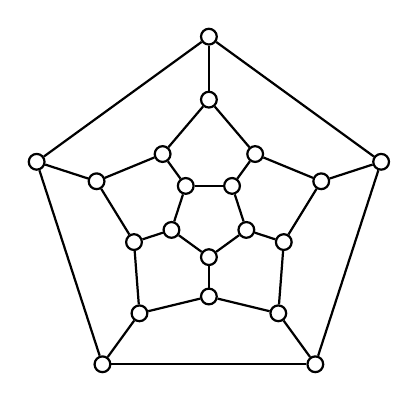
\begin{tikzpicture}[auto,
    specification/.style ={circle, draw, thick, inner sep = 0pt, minimum size=2mm}]
   \node[specification] (A)  at (18:2.3cm)  {};
   \node[specification] (B)  at (90:2.3cm)  {};
   \node[specification] (C)  at (162:2.3cm)  {};
   \node[specification] (D) at (234:2.3cm)  {};
   \node[specification] (E)  at (306:2.3cm)  {};
   \node[specification] (F)  at (18:1.5cm)  {};
   \node[specification] (G)  at (90:1.5cm)  {};
   \node[specification] (H)  at (162:1.5cm)  {};
   \node[specification] (I) at (234:1.5cm)  {};
   \node[specification] (J)  at (306:1.5cm)  {};
   \node[specification] (K)  at (-18:1.0cm)  {};
   \node[specification] (L)  at (-90:1.0cm)  {};
   \node[specification] (M)  at (-162:1.0cm)  {};
   \node[specification] (N) at (-234:1.0cm)  {};
   \node[specification] (O)  at (-306:1.0cm)  {};
   \node[specification] (P)  at (-18:0.5cm)  {};
   \node[specification] (Q)  at (-90:0.5cm)  {};
   \node[specification] (R)  at (-162:0.5cm)  {};
   \node[specification] (S) at (-234:0.5cm)  {};
   \node[specification] (T)  at (-306:0.5cm)  {};
   
   
   \draw[thick] (A) to  (B);
   \draw[thick] (B) to  (C);
   \draw[thick] (C) to  (D);
   \draw[thick] (D) to  (E);
   \draw[thick] (E) to  (A);
   \draw[thick] (A) to  (F);
   \draw[thick] (B) to  (G);
   \draw[thick] (C) to  (H);
   \draw[thick] (D) to  (I);
   \draw[thick] (E) to  (J);

   \draw[thick] (F) to  (O);
   \draw[thick] (O) to  (G);
   \draw[thick] (G) to  (N);
   \draw[thick] (N) to  (H);
   \draw[thick] (H) to  (M);
   \draw[thick] (M) to  (I);
   \draw[thick] (I) to  (L);
   \draw[thick] (L) to  (J);
   \draw[thick] (J) to  (K);
   \draw[thick] (K) to  (F);

   \draw[thick] (P) to  (K);
   \draw[thick] (Q) to  (L);
   \draw[thick] (R) to  (M);
   \draw[thick] (S) to  (N);
   \draw[thick] (T) to  (O);

   \draw[thick] (P) to  (Q);
   \draw[thick] (Q) to  (R);
   \draw[thick] (R) to  (S);
   \draw[thick] (S) to  (T);
   \draw[thick] (T) to  (P);
 \end{tikzpicture}
\end{Ex}


\begin{Ex}
  下图是否是哈密顿图?若是,找出一个哈密顿圈?若不是,说明理由。

  \centering
  
      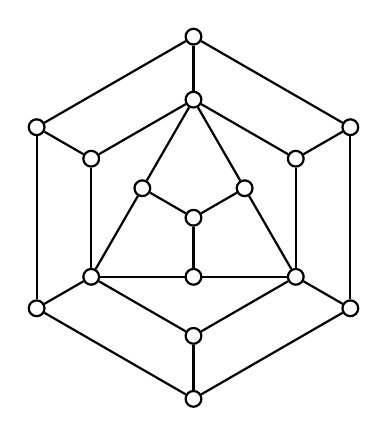
\begin{tikzpicture}[auto,
    specification/.style ={circle, draw, thick, inner sep = 0pt, minimum size=2mm}]
   \node[specification] (A)  at (30:2.3cm)  {};
   \node[specification] (B)  at (90:2.3cm)  {};
   \node[specification] (C)  at (150:2.3cm)  {};
   \node[specification] (D) at (210:2.3cm)  {};
   \node[specification] (E)  at (270:2.3cm)  {};
   \node[specification] (F)  at (330:2.3cm)  {};
   \node[specification] (G)  at (30:1.5cm)  {};
   \node[specification] (H)  at (90:1.5cm)  {};
   \node[specification] (I) at (150:1.5cm)  {};
   \node[specification] (J)  at (210:1.5cm)  {};
   \node[specification] (K)  at (270:1.5cm)  {};
   \node[specification] (L)  at (330:1.5cm)  {};
   \node[specification] (M)  at (30:0.75cm)  {};
   \node[specification] (N)  at (150:0.75cm)  {};
   \node[specification] (P)  at (270:0.75cm)  {};
   \node[specification] (Q)  at (0,0)  {};
   \draw[thick] (A) to  (B);
   \draw[thick] (B) to  (C);
   \draw[thick] (C) to  (D);
   \draw[thick] (D) to  (E);
   \draw[thick] (E) to  (F);
   \draw[thick] (F) to  (A);
   \draw[thick] (A) to  (G);
   \draw[thick] (B) to  (H);
   \draw[thick] (C) to  (I);
   \draw[thick] (D) to  (J);
   \draw[thick] (E) to  (K);
   \draw[thick] (F) to  (L);
   \draw[thick] (G) to  (H);
   \draw[thick] (H) to  (I);
   \draw[thick] (I) to  (J);
   \draw[thick] (J) to  (K);
   \draw[thick] (K) to  (L);
   \draw[thick] (L) to  (G);
   \draw[thick] (H) to  (M);
   \draw[thick] (M) to  (L);
   \draw[thick] (L) to  (P);
   \draw[thick] (P) to  (J);
   \draw[thick] (J) to  (N);
   \draw[thick] (N) to  (H);
   \draw[thick] (M) to  (Q);
   \draw[thick] (N) to  (Q);
   \draw[thick] (P) to  (Q);
 \end{tikzpicture}

\end{Ex}
\begin{Ex}
  下图是否是哈密顿图?若是,找出一个哈密顿圈?若不是,说明理由。

  \centering
  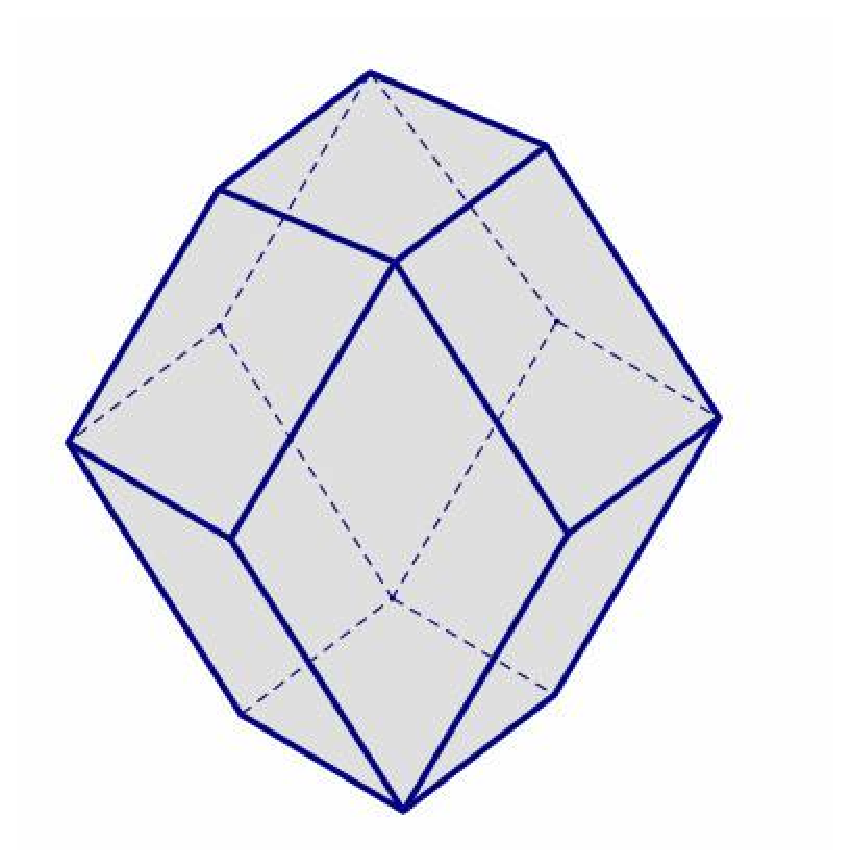
\includegraphics[width=5cm,height=4cm]{timg}

\end{Ex}

\begin{Ex}
  下图是否是哈密顿图?若是,找出一个哈密顿圈?若不是,说明理由。

  \centering
      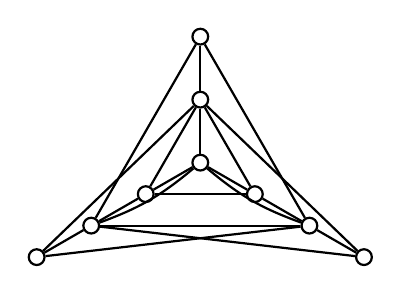
\begin{tikzpicture}[auto,
    specification/.style ={circle, draw, thick, inner sep = 0pt, minimum size=2mm}]
   \node[specification] (A)  at (90:1.6cm)  {};
   \node[specification] (B)  at (210:1.6cm)  {};
   \node[specification] (C)  at (330:1.6cm)  {};
   \node[specification] (D)  at (90:0.8cm)  {};
   \node[specification] (E)  at (210:0.8cm)  {};
   \node[specification] (F)  at (330:0.8cm)  {};
   \node[specification] (G)  at (210:2.4cm)  {};
   \node[specification] (H)  at (330:2.4cm)  {};
   \node[specification] (I)  at (0,0)  {};
   
   
   \draw[thick] (A) to  (B);
   \draw[thick] (B) to  (C);
   \draw[thick] (C) to  (A);
   \draw[thick] (D) to  (E);
   \draw[thick] (E) to  (F);
   \draw[thick] (F) to  (D);
   \draw[thick] (D) to  (G);
   \draw[thick] (D) to  (H);
   \draw[thick] (H) to  (B);
   \draw[thick] (G) to  (C);
   \draw[thick] (A) to  (D);
   \draw[thick] (C) to  (F);
   \draw[thick] (B) to  (E);
   \draw[thick] (I) to  (D);
   \draw[thick] (I) to  (E);
   \draw[thick] (I) to  (F);
   \draw[thick] (G) to  (B);
   \draw[thick] (H) to  (C);
   \draw[thick] (B) to [bend right = 10] (I);
   \draw[thick] (C) to [bend left = 10] (I);
 \end{tikzpicture}


\end{Ex}


\begin{Ex}
  下图是否是哈密顿图?若是,找出一个哈密顿圈?若不是,说明理由。

\centering  
      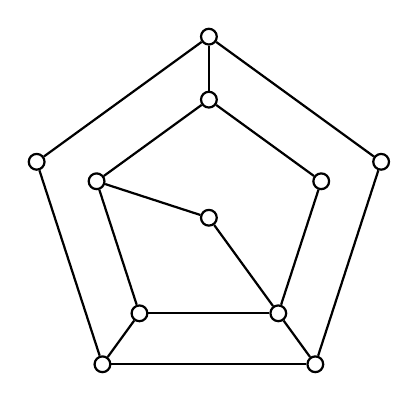
\begin{tikzpicture}[auto,
    specification/.style ={circle, draw, thick, inner sep = 0pt, minimum size=2mm}]
   \node[specification] (A)  at (18:2.3cm)  {};
   \node[specification] (B)  at (90:2.3cm)  {};
   \node[specification] (C)  at (162:2.3cm)  {};
   \node[specification] (D) at (234:2.3cm)  {};
   \node[specification] (E)  at (306:2.3cm)  {};
   \node[specification] (F)  at (18:1.5cm)  {};
   \node[specification] (G)  at (90:1.5cm)  {};
   \node[specification] (H)  at (162:1.5cm)  {};
   \node[specification] (I) at (234:1.5cm)  {};
   \node[specification] (J)  at (306:1.5cm)  {};
   \node[specification] (K)  at (0,0)  {};
   
   
   
   \draw[thick] (A) to  (B);
   \draw[thick] (B) to  (C);
   \draw[thick] (C) to  (D);
   \draw[thick] (D) to  (E);
   \draw[thick] (E) to  (A);
   
   \draw[thick] (F) to  (G);
   \draw[thick] (G) to  (H);
   \draw[thick] (H) to  (I);
   \draw[thick] (I) to  (J);
   \draw[thick] (J) to  (F);
   
   \draw[thick] (B) to  (G);
   \draw[thick] (D) to  (I);
   \draw[thick] (E) to  (J);
   \draw[thick] (K) to  (H);
   \draw[thick] (K) to  (J);

 \end{tikzpicture}
\end{Ex}

\begin{Ex}
  下图是否是哈密顿图?若是,找出一个哈密顿圈?若不是,说明理由。

  \centering
      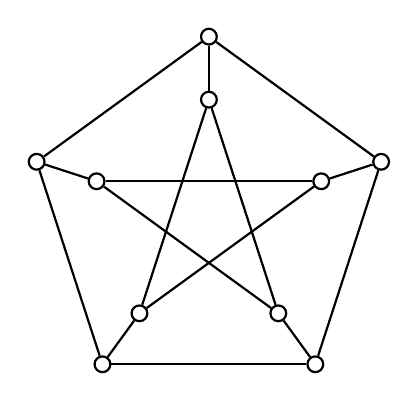
\begin{tikzpicture}[auto,
    specification/.style ={circle, draw, thick, inner sep = 0pt, minimum size=2mm}]
   \node[specification] (A)  at (18:2.3cm)  {};
   \node[specification] (B)  at (90:2.3cm)  {};
   \node[specification] (C)  at (162:2.3cm)  {};
   \node[specification] (D) at (234:2.3cm)  {};
   \node[specification] (E)  at (306:2.3cm)  {};
   \node[specification] (F)  at (18:1.5cm)  {};
   \node[specification] (G)  at (90:1.5cm)  {};
   \node[specification] (H)  at (162:1.5cm)  {};
   \node[specification] (I) at (234:1.5cm)  {};
   \node[specification] (J)  at (306:1.5cm)  {};
   
   
   \draw[thick] (A) to  (B);
   \draw[thick] (B) to  (C);
   \draw[thick] (C) to  (D);
   \draw[thick] (D) to  (E);
   \draw[thick] (E) to  (A);
   \draw[thick] (A) to  (F);
   \draw[thick] (B) to  (G);
   \draw[thick] (C) to  (H);
   \draw[thick] (D) to  (I);
   \draw[thick] (E) to  (J);
   \draw[thick] (G) to  (I);
   \draw[thick] (I) to  (F);
   \draw[thick] (F) to  (H);
   \draw[thick] (H) to  (J);
   \draw[thick] (J) to  (G);

 \end{tikzpicture}
\end{Ex}


\begin{Ex}
  以下4个图中,存在一个哈密顿圈的是$\underline{\quad\quad}$。
  \vspace{0.5cm}

  A.
    \begin{minipage}{0.18\linewidth}
    \centering
    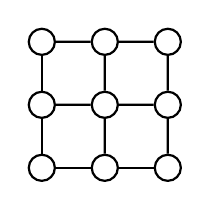
\begin{tikzpicture}[auto,
    specification/.style ={circle, draw, thick}, scale = 0.8]
   \node[specification] (A)  at (0,0)  {};
   \node[specification] (B)  at (1,0)  {};
   \node[specification] (C)  at (2,0)  {};
   \node[specification] (D)  at (0,1)  {};
   \node[specification] (E)  at (1,1)  {};
   \node[specification] (F)  at (2,1)  {};
   \node[specification] (G)  at (0,2)  {};
   \node[specification] (H)  at (1,2)  {};
   \node[specification] (I)  at (2,2)  {};

   \draw[thick] (A) to  (B);
   \draw[thick] (B) to  (C);
   \draw[thick] (D) to  (E);
   \draw[thick] (E) to  (F);
   \draw[thick] (G) to (H);
   \draw[thick] (H) to (I);
   \draw[thick] (A) to (D);
   \draw[thick] (B) to (E);
   \draw[thick] (C) to (F);
   \draw[thick] (D) to (G);
   \draw[thick] (E) to (H);
   \draw[thick] (F) to (I);
 \end{tikzpicture}
\end{minipage}\hfill
  B.
    \begin{minipage}{0.18\linewidth}
    \centering
    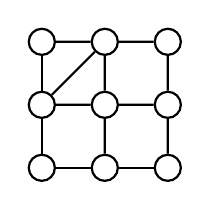
\begin{tikzpicture}[auto,
    specification/.style ={circle, draw, thick}, scale = 0.8]
   \node[specification] (A)  at (0,0)  {};
   \node[specification] (B)  at (1,0)  {};
   \node[specification] (C)  at (2,0)  {};
   \node[specification] (D)  at (0,1)  {};
   \node[specification] (E)  at (1,1)  {};
   \node[specification] (F)  at (2,1)  {};
   \node[specification] (G)  at (0,2)  {};
   \node[specification] (H)  at (1,2)  {};
   \node[specification] (I)  at (2,2)  {};

   \draw[thick] (A) to  (B);
   \draw[thick] (B) to  (C);
   \draw[thick] (D) to  (E);
   \draw[thick] (E) to  (F);
   \draw[thick] (G) to (H);
   \draw[thick] (H) to (I);
   \draw[thick] (A) to (D);
   \draw[thick] (B) to (E);
   \draw[thick] (C) to (F);
   \draw[thick] (D) to (G);
   \draw[thick] (E) to (H);
   \draw[thick] (F) to (I);
   \draw[thick] (D) to (H);

 \end{tikzpicture}
\end{minipage}\hfill
      C.
    \begin{minipage}{0.18\linewidth}
    \centering
    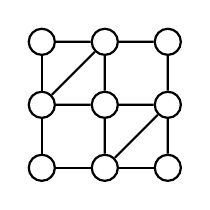
\begin{tikzpicture}[auto,
    specification/.style ={circle, draw, thick}, scale=0.8]
   \node[specification] (A)  at (0,0)  {};
   \node[specification] (B)  at (1,0)  {};
   \node[specification] (C)  at (2,0)  {};
   \node[specification] (D)  at (0,1)  {};
   \node[specification] (E)  at (1,1)  {};
   \node[specification] (F)  at (2,1)  {};
   \node[specification] (G)  at (0,2)  {};
   \node[specification] (H)  at (1,2)  {};
   \node[specification] (I)  at (2,2)  {};

   \draw[thick] (A) to  (B);
   \draw[thick] (B) to  (C);
   \draw[thick] (D) to  (E);
   \draw[thick] (E) to  (F);
   \draw[thick] (G) to (H);
   \draw[thick] (H) to (I);
   \draw[thick] (A) to (D);
   \draw[thick] (B) to (E);
   \draw[thick] (C) to (F);
   \draw[thick] (D) to (G);
   \draw[thick] (E) to (H);
   \draw[thick] (F) to (I);
   \draw[thick] (D) to (H);
   \draw[thick] (B) to (F);
 \end{tikzpicture}
\end{minipage}\hfill
      D.
    \begin{minipage}{0.18\linewidth}
    \centering
    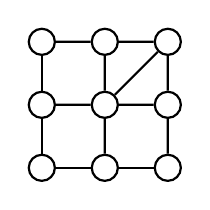
\begin{tikzpicture}[auto,
    specification/.style ={circle, draw, thick}, scale=0.8]
   \node[specification] (A)  at (0,0)  {};
   \node[specification] (B)  at (1,0)  {};
   \node[specification] (C)  at (2,0)  {};
   \node[specification] (D)  at (0,1)  {};
   \node[specification] (E)  at (1,1)  {};
   \node[specification] (F)  at (2,1)  {};
   \node[specification] (G)  at (0,2)  {};
   \node[specification] (H)  at (1,2)  {};
   \node[specification] (I)  at (2,2)  {};

   \draw[thick] (A) to  (B);
   \draw[thick] (B) to  (C);
   \draw[thick] (D) to  (E);
   \draw[thick] (E) to  (F);
   \draw[thick] (G) to (H);
   \draw[thick] (H) to (I);
   \draw[thick] (A) to (D);
   \draw[thick] (B) to (E);
   \draw[thick] (C) to (F);
   \draw[thick] (D) to (G);
   \draw[thick] (E) to (H);
   \draw[thick] (F) to (I);
   \draw[thick] (E) to (I);

 \end{tikzpicture}
\end{minipage}\hfill

\end{Ex}

\begin{Ex}
  以下4个图中,不存在哈密顿路的是$\underline{\quad\quad}$。
  \vspace{0.5cm}

  A.
    \begin{minipage}{0.18\linewidth}
    \centering
    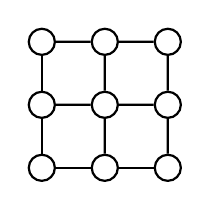
\begin{tikzpicture}[auto,
    specification/.style ={circle, draw, thick}, scale = 0.8]
   \node[specification] (A)  at (0,0)  {};
   \node[specification] (B)  at (1,0)  {};
   \node[specification] (C)  at (2,0)  {};
   \node[specification] (D)  at (0,1)  {};
   \node[specification] (E)  at (1,1)  {};
   \node[specification] (F)  at (2,1)  {};
   \node[specification] (G)  at (0,2)  {};
   \node[specification] (H)  at (1,2)  {};
   \node[specification] (I)  at (2,2)  {};

   \draw[thick] (A) to  (B);
   \draw[thick] (B) to  (C);
   \draw[thick] (D) to  (E);
   \draw[thick] (E) to  (F);
   \draw[thick] (G) to (H);
   \draw[thick] (H) to (I);
   \draw[thick] (A) to (D);
   \draw[thick] (B) to (E);
   \draw[thick] (C) to (F);
   \draw[thick] (D) to (G);
   \draw[thick] (E) to (H);
   \draw[thick] (F) to (I);
 \end{tikzpicture}
\end{minipage}\hfill
  B.
    \begin{minipage}{0.18\linewidth}
    \centering
    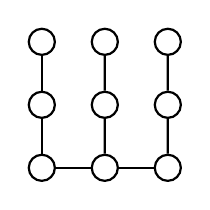
\begin{tikzpicture}[auto,
    specification/.style ={circle, draw, thick}, scale = 0.8]
   \node[specification] (A)  at (0,0)  {};
   \node[specification] (B)  at (1,0)  {};
   \node[specification] (C)  at (2,0)  {};
   \node[specification] (D)  at (0,1)  {};
   \node[specification] (E)  at (1,1)  {};
   \node[specification] (F)  at (2,1)  {};
   \node[specification] (G)  at (0,2)  {};
   \node[specification] (H)  at (1,2)  {};
   \node[specification] (I)  at (2,2)  {};

   \draw[thick] (A) to  (B);
   \draw[thick] (B) to  (C);
   \draw[thick] (A) to (D);
   \draw[thick] (B) to (E);
   \draw[thick] (C) to (F);
   \draw[thick] (D) to (G);
   \draw[thick] (E) to (H);
   \draw[thick] (F) to (I);

 \end{tikzpicture}
\end{minipage}\hfill
      C.
    \begin{minipage}{0.18\linewidth}
    \centering
    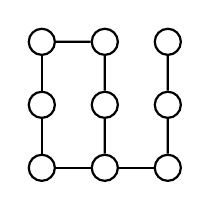
\begin{tikzpicture}[auto,
    specification/.style ={circle, draw, thick}, scale=0.8]
   \node[specification] (A)  at (0,0)  {};
   \node[specification] (B)  at (1,0)  {};
   \node[specification] (C)  at (2,0)  {};
   \node[specification] (D)  at (0,1)  {};
   \node[specification] (E)  at (1,1)  {};
   \node[specification] (F)  at (2,1)  {};
   \node[specification] (G)  at (0,2)  {};
   \node[specification] (H)  at (1,2)  {};
   \node[specification] (I)  at (2,2)  {};

   \draw[thick] (A) to  (B);
   \draw[thick] (B) to  (C);
   \draw[thick] (A) to (D);
   \draw[thick] (B) to (E);
   \draw[thick] (C) to (F);
   \draw[thick] (D) to (G);
   \draw[thick] (E) to (H);
   \draw[thick] (F) to (I);
   \draw[thick] (G) to (H);
 \end{tikzpicture}
\end{minipage}\hfill
      D.
    \begin{minipage}{0.18\linewidth}
    \centering
    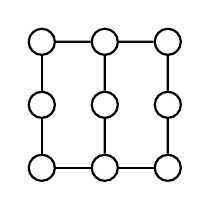
\begin{tikzpicture}[auto,
    specification/.style ={circle, draw, thick}, scale=0.8]
   \node[specification] (A)  at (0,0)  {};
   \node[specification] (B)  at (1,0)  {};
   \node[specification] (C)  at (2,0)  {};
   \node[specification] (D)  at (0,1)  {};
   \node[specification] (E)  at (1,1)  {};
   \node[specification] (F)  at (2,1)  {};
   \node[specification] (G)  at (0,2)  {};
   \node[specification] (H)  at (1,2)  {};
   \node[specification] (I)  at (2,2)  {};

      \draw[thick] (A) to  (B);
   \draw[thick] (B) to  (C);
   \draw[thick] (A) to (D);
   \draw[thick] (B) to (E);
   \draw[thick] (C) to (F);
   \draw[thick] (D) to (G);
   \draw[thick] (E) to (H);
   \draw[thick] (F) to (I);
   \draw[thick] (G) to (H);
   \draw[thick] (H) to (I);

 \end{tikzpicture}
\end{minipage}\hfill



\end{Ex}


%%% Local Variables:
%%% mode: latex
%%% TeX-master: "book"
%%% End:
